\section{Informationstheorie und Quellencodierung \formelbuch{245-10}}
\subsection{DMS - Discrete Memoryless Source}
Eine Informations\textbf{quelle} ist ein Objekt welches \textbf{Ereignise}, welche zufällig aus einer
WSK-Dichtefunktion ausgewählt werden, \textbf{generiert}. \\ 
Eine diskrete Quelle hat einen endlichen \textbf{Satz an Symbolen}, welcher auch \textbf{Alphabet}
genannt wird. Die Elemente dieses Satzes nennt man \textbf{Symbole} oder \textbf{Zeichen}. \\
Wird ein Symbol unabhängig vom Vorherigen generiert, so handelt es sich um eine DMS (diskrete
gedächtnisfreie Quelle). Eine solche wird mit folgenden Eigenschaften charakterisiert:
%\renewcommand{\parskip}{0}
\begin{itemize}\addtolength{\itemsep}{-0.3\baselineskip}
  \item Liste der Symbole - Alphabet
  \item Auftretenswahrscheinlichkeiten dieser Symbole - WSK-Dichtefunktion
  \item Symbolrate 
\end{itemize} 

\skriptsubsubsection{Informationsgehalt, Binary Unit, Entropie, Informationsrate}{246-10.2-B.1,2,3}
Mathematisch gesehen kann man sagen, je \textbf{unwahrscheinlicher} das \textbf{Eintreten} eines \textbf{spezifischen
Ereignisses} ist, desto \textbf{grösser} ist dessen \textbf{Informationsgehalt}.

\begin{multicols}{2}
\renewcommand{\arraystretch}{\arraystretchOriginal}
\begin{tabular}{|l|l|l|}
	\hline
	\textbf{Grösse}	& \textbf{Bezeichnung}	& \textbf{Einheit} \\ 
	\hline
	$I(x_i)$ 	& Informationsgehalt 	& b \\
	\hline
	$P(x_i)$	& Auftretens-WSK eines Symbols & \\
	\hline
	$H(x_i)$	& Entropie				& b/Symbol\\
	\hline
	$R$			& Informationsrate 		& b/s \\
	\hline
	$r$			& Symbolrate/Bitrate	& Symbole/s	 \\
	\hline
\end{tabular}

Der Informationsgehalt kann in folgenden Masseinheiten angegeben werden:
\[ [I(X)] = \begin{cases}
            	\text{bit (\emph{bi}nary uni\emph{t})} 
            		& \text{falls } base=2. \\
            	\text{hartley oder decit}
            		& \text{falls } base=10. \\
            	\text{nat (\emph{na}tural uni\emph{t})} 
            		& \text{falls } base=e
			\end{cases} 
\]
\textbf{Standardmässig} verwenden wir $base=2$, also bit oder gekürzt
\textbf{b}. Binary Unit ist ein Mass für den Informationsgehalt und sollte nicht mit dem Term ``bit'' (Binäres Zeichen) verwechselt
werden.
\end{multicols}

\begin{align*}
	I(x_i)	&= \log_{base} \frac{1}{P(x_i)} = - \log_{base} P(x_i) \\
	R		&= r H (X) \\
	H(X)	&= E[I(x_i)] = \sum\limits_{i=1}^m P(x_i) I(x_i) = - \sum\limits_{i=1}^m P(x_i) \log_2{P(x_i)} \qquad 0 \leq H(x) \leq \log_2(m) \\
	H(X|Y)	&=- \sum\limits_{j=1}^{n} \sum\limits_{i=1}^{m} P(x_i,y_j) log_2(P(x_i|y_j)) \\
	H(X,Y)	&=- \sum\limits_{j=1}^{n} \sum\limits_{i=1}^{m} P(x_i,y_j) log_2(P(x_i,y_j)) \\
	I(X;Y)	&=I(Y;X)=H(X)+H(Y)-H(X,Y)=H(X)-H(X|Y) 
\end{align*}


\skriptsubsection{DMC - Discrete Memoryless Channels}{247-10.3}
\begin{minipage}{9.5cm}
	\begin{center}
		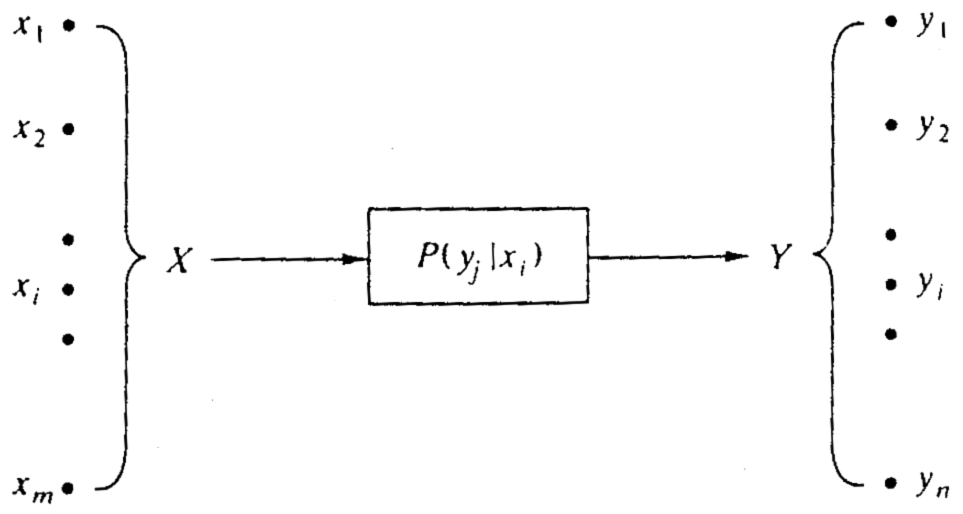
\includegraphics[width=7.5cm]{../NaT2/bilder/10_DMC.png}
	\end{center}
\end{minipage}
\begin{minipage}{8.5cm}
	Ein DMC (diskreter gedächtnisfreier Kanal) ist ein statistisches Modell mit Eingang $X$ und
	Ausgang $Y$. \\ \\
	Er besitzt \textbf{$m$ Eingänge} und \textbf{$n$ Ausgänge}. \\ \\
	Alle Auftretenswahrscheinlichkeiten $P(x_i)$ der einzelnen Eingangs-Symbole werden als gegeben
	betrachtet. \\
	Jeder Übertragungspfad ist durch die Kanal-Übertragungs-Wahrscheinlichkeiten (channel transition
	probabilities) $P(y_j | x_i)$ definiert.
\end{minipage}

\subsubsection{Darstellung in Matritzenform}
\begin{minipage}{9cm}
	\textbf{Kanalmatrix}
	$$ \boxed{[P(Y | X)] = \begin{bmatrix}
              P(y_1 | x_1) & P(y_2 | x_1) & \ldots & P(y_n | x_1) \\
              P(y_1 | x_2) & P(y_2 | x_2) & \ldots & P(y_n | x_2) \\
             . & . & . & . \\
              P(y_1 | x_m) & P(y_2 | x_m) & \ldots & P(y_n | x_m)
           \end{bmatrix}}$$ \\
	$ [P(Y)] = [P(y_1) \quad P(y_2) \quad \ldots \quad P(y_n)] = [P(X)] \cdot [P(Y|X)]$ \\
%	$ [P(Y)] =  \\
	$ [P(X)] = [P(x_1) \quad P(x_2) \quad \ldots \quad P(x_m)]$ \\ \\
	$\sum\limits_{j=1}^n P(y_j | x_i) = 1 (\forall i)$ \qquad $\sum$ jeder Zeile von $[P(Y|X)]=1$\\ \\
\end{minipage}
\begin{minipage}{9cm}
	\textbf{Verbundmatrix}
	\begin{center}$ \boxed{[P(Y,X)] = \begin{bmatrix}
              P(y_1, x_1) & P(y_2, x_1) & \ldots & P(y_n, x_1) \\
              P(y_1, x_2) & P(y_2, x_2) & \ldots & P(y_n, x_2) \\
             . & . & . & . \\
              P(y_1, x_m) & P(y_2, x_m) & \ldots & P(y_n, x_m)
           \end{bmatrix}}$
	\end{center}
	$  [P(Y,X)] =  \begin{bmatrix}
    	P(x_1) & 0 & \ldots & 0 \\
    	0 & P(x_2) & \ldots & 0 \\
    	. & . & . & . \\
    	0 & 0 & \ldots & P(x_m)
    \end{bmatrix} [P(Y|X)] $\\ 
	Elemente auf der Diagonale sollten den grössten Wert gegenüber anderen Elementen auf der Zeile
	besitzen. \\
	$\sum $ aller Elemente von $[P(Y,X)] = 1$
\end{minipage}

\skriptsubsubsection{Spezielle Kanäle}{248-10.3.C}
\textbf{Verlustfreier (lossless) Kanal} \\
\begin{minipage}{14cm}
	Auf jeder Spalte der Kanalmatrix gibt es jeweils nur ein  Element $\neq 0$. \\

	$$ [P(Y | X)] = \begin{bmatrix}
              \frac34 & \frac14 & 0 & 0 & 0 \\
              0 & 0 & \frac13 & \frac23 & 0 \\
              0 & 0 & 0 & 0 & 1
           \end{bmatrix}$$ \\
\end{minipage}
\begin{minipage}{4cm}
\begin{center}
	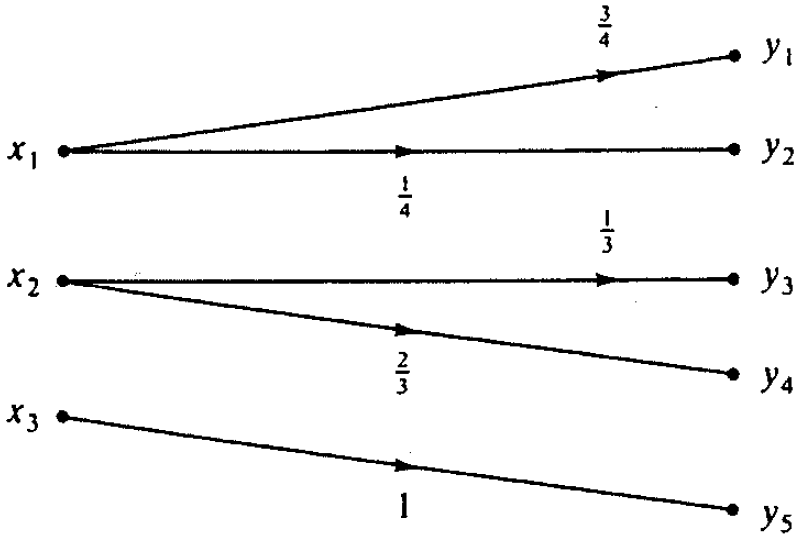
\includegraphics[height=3cm]{../NaT2/bilder/10_channels_lossless.png}
\end{center}
\end{minipage}

\textbf{Deterministischer (deterministic) Kanal} \\
\begin{minipage}{14cm}
	Auf jeder Zeile der Kanalmatrix gibt es jeweils nur ein  Element $\neq 0$, welches $1$ sein
	muss.

	$$ [P(Y | X)] = \begin{bmatrix}
           		1 & 0 & 0 \\
           		1 & 0 & 0 \\
           		0 & 1 & 0 \\
           		0 & 1 & 0 \\
           		0 & 0 & 1
           \end{bmatrix}$$
\end{minipage}
\begin{minipage}{4cm}
\begin{center}
	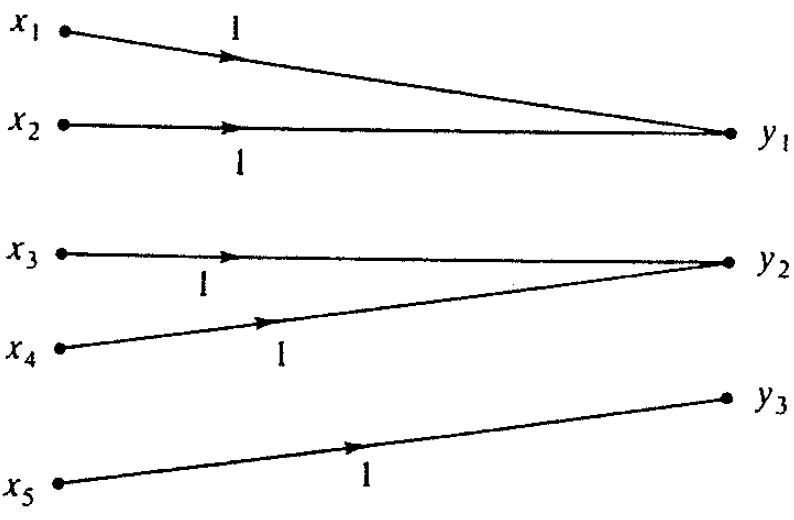
\includegraphics[height=3cm]{../NaT2/bilder/10_channels_deterministic.png}
\end{center}
\end{minipage}

\textbf{Rauschfreier (noiseless) Kanal} \\
\begin{minipage}{14cm}
	Die Kanalmatrix entspricht der Einheitsmatrix.

	$$ [P(Y | X)] = \begin{bmatrix}
           		1 & 0 & \ldots & 0\\
           		0 & 1 & \ldots & 0\\
           		\vdots & \vdots & \vdots & \vdots \\
           		0 & 0 & \ldots & 1\\
           \end{bmatrix} = I$$ \\
\end{minipage}
\begin{minipage}{4cm}
\begin{center}
	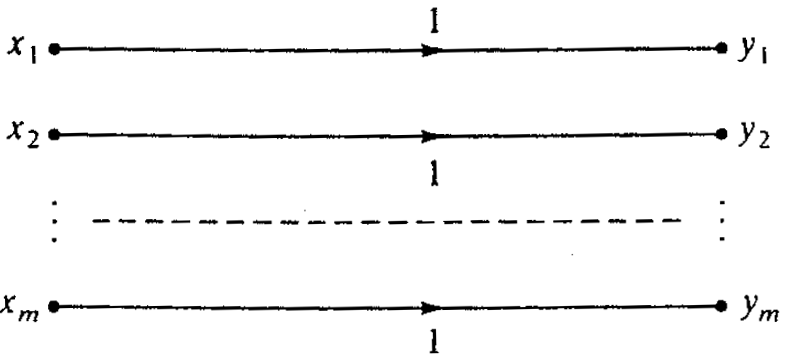
\includegraphics[width=4.5cm]{../NaT2/bilder/10_channels_noiseless.png}
\end{center}
\end{minipage}

\textbf{Binärer Symmetrischer (binary symmetrical) Kanal} \\
\begin{minipage}{14cm}

	$$ [P(Y | X)] = \begin{bmatrix}
           		1-p_e & p_e \\
           		p_e & 1-p_e
           \end{bmatrix} $$
\end{minipage}
\begin{minipage}{4cm}
\begin{center}
	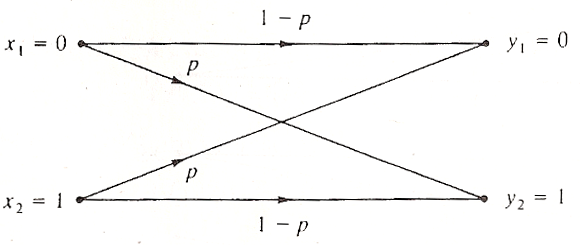
\includegraphics[width=4.5cm]{../NaT2/bilder/10_channels_binarysymmetrical.png}
\end{center}
\end{minipage}




% \skriptsubsection{Gegenseitige (mutual) Information}{250-10.4}
%  TODO \subsubsection{Bedingte Entropien}
%
%  TODO \subsubsection{Gegenseitige Information}
% \textbf{TODO}

\skriptsubsection{Kanalkapazität}{251-10.5}
\begin{minipage}[c]{8cm}
	$$ C_s = \max\limits_{\{ P(x_i) \}}{I (X; Y)} $$
	$$ C = r_b C_s $$
	$$ r_s H(X) \leq C$$
\end{minipage}
\begin{minipage}[c]{10cm}
	$C_s$ Kanalkapazität pro Symbol, $[C_s]$ = b/Symbol \\
	$C$ Kanalkapazität pro Sekunde, $[C]$ = b/s \\
	$r_s$ Symbolrate Quelle, $r_b$ Bitrate Kanal, $[r]$ = Symbol/s \\
	Bedingung für eine (theoretisch) fehlerfreie Übertragung
\end{minipage}

\subsubsection{Kanalkapazitätien spezieller Kanäle}

	\renewcommand{\arraystretch}{2}
	\begin{tabular}{| p{3.5cm} | p{7.5cm} | p{6.5cm} |}
		\hline  
    		\textbf{Verlustfrei}
    			& $ I(X; Y) = H(X) $
    			& $ C_s = \max\limits_{\{ P(x_i) \}}{H (X)} = \log_2 m $ \\
		\hline
    		\textbf{Deterministisch}
    			& $ I(X; Y) = H(Y) $
    			& $ C_s = \max\limits_{\{ P(x_i) \}}{H (Y)} = \log_2 n $ \\
		\hline
    		\textbf{Rauschfrei}
    			& $ I(X; Y) = H(Y) = H(X)$
    			& $ C_s = \log_2 n = \log_2 m$ \\
		\hline
    		\textbf{Binär Symmetrisch}
    			& $ I(X; Y) = H(Y) + p_e \log_2 p_e + (1-p_e) \log_2 (1-p_e)$
    			& $ C_s = 1 + p_e \log_2 p_e + (1-p_e) \log_2 (1-p_e)$ \\
		\hline
    		\textbf{AWGN}
    			& $ C = 2 B C_s = B \log_2 (1 + \left(\frac{S}{N}\right)_0)$ 
    			& $ C_s = \max{I(X; Y) = \frac{1}{2} \log_2 (1 + \left(\frac{S}{N}\right)_0)}$ \\
		\hline
 	\end{tabular}
	\renewcommand{\arraystretch}{1} \\ \\
Wobei $B$ der Bandbreite des Kanals entspricht. 
% \skriptsubsection{AWGN-Channel}{252-10.6}
% \textbf{TODO}

\skriptsubsection{Quellencodierung}{253-10.7}

\skriptsubsubsection{Code-Länge, -Effizienz, -Redundanz}{253-10.7.A/B}
Gilt für eine DMS mit endlicher Entropie. \\

\begin{minipage}[c]{8cm}
	$$ L = \sum\limits_{i=1}^m P(x_i) n_i $$
	$$ \eta = \frac{H(x)}{L} = \frac{L_{min}}{L} \qquad \qquad  \gamma_c = 1 -
	\eta $$
	$$ \gamma_q = R(x) = H_{max} - H(x) = \log_2(m) - H(x)$$
\end{minipage}
\begin{minipage}[c]{10cm}
	$L$ Durchschnittliche Codewort-Länge, $[L]$ = Bits/Symbol \\
	$L_{min}$ kleinstmölgliches L \\
	$P(x_i)$ Auftretenswahrscheinlichkeit des Symbols \\
	$n_i$ Symbollänge, $[n_i] = $ Bits \\
	$m$ Anzahl Symbole des Codes \\
	$\eta$ Effizienz \\
	$\gamma_c$ Redundanz des Codes; $\gamma_q = R(x)$ Redundanz der Quelle \\
	$H(X)$ Entropie, $[H(X)] = $ b/Symbol 
\end{minipage}
% TODO: Redundanz mit H(X) und Hmax 

\skriptsubsubsection{Klassifizierung von Codes}{254-10.7.C}
	\renewcommand{\arraystretch}{2}
	\begin{tabular}{| p{6cm} | p{12cm} |}
		\hline
    	\textbf{Bezeichnung} & \textbf{Eigenschaften}  \\
		\hline  
    	\begin{minipage}[c]{6cm}  
	    	\textbf{Fixed Lengh Code} \\
	    	feste Länge 
      	\end{minipage}
    	& \begin{minipage}[c]{12cm}    
	    		Alle Codewörter haben die gleiche Länge. \\
	    		Bsp.: ASCII-Code. 
      	\end{minipage}
    	\\
		\hline
    	\begin{minipage}[c]{6cm}    
    		\textbf{Variable Lengh Code} \\
    		variable Länge 
      	\end{minipage}
    	& \begin{minipage}[c]{12cm}    
    		Codewörter haben unterschiedliche Länge. \\
    		Bsp.: Shannon-Fano, Huffman und Morse Code. 
      	\end{minipage}
    	\\
		\hline
    	\begin{minipage}[c]{6cm}    
    		\textbf{Prefix-Free Code} \\
    		präfixfrei 
      	\end{minipage}
    	& \begin{minipage}[c]{12cm}    
    		Kein Codewort dient als Präfix (Vorsible) für ein anderes Codewort. \\
    		Bsp.: Shannon-Fano oder Huffman Code, aber nicht Morse-Code. 
      	\end{minipage}
    	\\
		\hline
    	\begin{minipage}[c]{6cm}    
    		\textbf{Uniquely Decodeable Code} \\
    		eindeutig decodierbar 
      	\end{minipage}
    	& \begin{minipage}[c]{12cm}    
    		Kette von Codewörtern kann eindeutig wieder in die ursrünglichen Symbolfolgen
    		zurückgewandelt werden. \\
    		Präfixfreie Codes sind eindeutig decodierbar. 
      	\end{minipage}
    	\\
		\hline
    	\begin{minipage}[c]{6cm}    
    		\textbf{Instantaneous Code} \\
    		sofort decodierbar 
      	\end{minipage}
    	& \begin{minipage}[c]{12cm}    
    		Liefert nach Empfang jedes einzelnen Codeworts sofort ein eindeutiges Symbol. \\
    		Jeder Instantaneous Code mit minimaler Codelänge ist optimaler Code. 
      	\end{minipage}
    	\\
		\hline
    	\begin{minipage}[c]{6cm}    
    		\textbf{Optimal Code}  
      	\end{minipage}
    	& \begin{minipage}[c]{12cm}    
    		$\eta = 1 = 100 \% $ 
      	\end{minipage}
    	\\
		
		\hline
 	\end{tabular}
	\renewcommand{\arraystretch}{1}

\skriptsubsubsection{Kraft'sche Ungleichung}{255-10.7.D}
Wenn diese Ungleichung erfüllt ist, besagt sie, dass ein \textbf{eindeutig} und \textbf{sofort
decodierbarer} Code gefunden werden kann. \\
Gegeben ist eine Quelle mit \textbf{Alphabet $x_i$} der \textbf{Länge $m$}, wobei jedem
\textbf{Symbol $x_i$} kein Codewort aber eine \textbf{Codelänge $n_i$} zugewiesen ist.
$$ K = \sum\limits_{i=1}^{m} 2 ^{-n_i} \leq 1$$ 
Die Kraft'sche Ungleichung hilft jedoch zum Auffinden dieses Codes nicht weiter.

\skriptsubsection{Entropie Codierung}{255-10.8}
\textbf{Ziel:} Durchschnittliche Codelänge an Entropie annähern $ \Rightarrow $ Wirkungsgrad
steigern.

\skriptsubsubsection{Shannon - Fanno Codierung}{255-10.8.A}
\begin{multicols}{2}
	\begin{tabular}{|c|c|c|c|c|c|l|}
		\hline
		$x_i$	& $P(x_i)$ 	& Step 1	& Step 2	& Step 3 	& Step 4 	& Code \\
		\hline
		$x_1$	& 0.30		& 0			& 0			& 			&			& 00 \\
		\cline{4-4}
		$x_2$	& 0.25		& 0			& 1			& 			& 			& 01 \\
		\cline{3-4}
		$x_3$	& 0.20		& 1			& 0			& 			& 			& 10 \\
		\cline{4-5}
		$x_4$	& 0.12		& 1			& 1			& 0			& 			& 110 \\
		\cline{5-6}
		$x_5$	& 0.08		& 1			& 1			& 1			& 0			& 1110 \\
		\cline{6-6}		
		$x_6$	& 0.05		& 1			& 1			& 1			& 1			& 1111 \\
		\hline 
	\end{tabular}
	
	\begin{enumerate}
		\item Symbole mit \textbf{absteigender} Wahrscheinlichkeit anordnen.
		\item Trennung in \textbf{2 Teilmengen} mit möglichst gleicher WSK.
		\item \textbf{Obere} Teilmenge Symbol \textbf{0}, \textbf{unterer} Teilmenge Symbol \textbf{1}
		  zuordnen.
		\item Weiterhin unterteilen gemäss obigen Schritten, bis keine Teilung mehr möglich ist.
	\end{enumerate}
\end{multicols}



\skriptsubsubsection{Huffman Codierung}{256-10.8.B}
\begin{multicols}{2}
  \adjustbox{width=\linewidth, frame}{\begin{tikzpicture}[every node/.style={minimum height=2em}]
\matrix [matrix of math nodes](Mat)
{
x_i  &|[minimum width=1.5em]|& P(x_i) &|[minimum width=4em]| Code &       &|[minimum width=4em]|      &       &|[minimum width=4em]|  &   &|[minimum width=4em]|  &   &\\
x_1 &&0.30	&	& 0.30  &   &0.30   &   &0.45&  &0.55&\\
x_2 && 0.25	&	& 0.25  &   &0.25   &   &0.30&  &0.45&\\
x_3 && 0.20	&	& 0.20  &   &0.25   &   &0.25&  &   &\\
x_4 && 0.12	&	& 0.13   &   &0.20   &   &   &   &   &\\
x_5 && 0.08	&	& 0.12   &   &       &   &   &   &   &\\
x_6 && 0.05	&	&   &   &       &   &   &   &   &\\
};

\draw (Mat-2-3) -- (Mat-2-5) node[above=-0.1,midway]{00};
\draw (Mat-3-3) -- (Mat-3-5) node[above=-0.1,midway]{01};
\draw (Mat-4-3) -- (Mat-4-5) node[above=-0.1,midway]{11};
\draw (Mat-2-5) -- (Mat-2-7) node[above=-0.1,midway]{00};
\draw (Mat-3-5) -- (Mat-3-7) node[above=-0.1,midway]{01};

\draw(Mat-5-3.east) --++(1em,0) -- (Mat-6-5.west)node[above,pos=0.2]{101};
\draw(Mat-4-5.east) --++(1em,0) -- (Mat-5-7.west)node[above,pos=0.2]{11};
\draw(Mat-2-7.east) --++(1em,0) -- (Mat-3-9.west)node[above,pos=0.2]{00};
\draw(Mat-3-7.east) --++(1em,0) -- (Mat-4-9.west)node[above,pos=0.2]{01};
\draw(Mat-2-9.east) --++(1em,0) -- (Mat-3-11.west)node[above,pos=0.2]{1};

\draw (Mat-6-3.east)-|node[above=-0.1,pos=0.3]{1000}++(2em,-1em) coordinate(aa) --++(1em,0) |- (Mat-5-5.west);
\draw (Mat-7-3.east)-|node[below=-0.1,pos=0.3]{1001} (aa);

\draw (Mat-5-5.east)-|node[above=-0.1,pos=0.3]{100}++(2em,-1em) coordinate(bb) --++(1em,0) |- (Mat-4-7.west);
\draw (Mat-6-5.east)-|node[below=-0.1,pos=0.3]{101} (bb);

\draw (Mat-4-7.east)-|node[above=-0.1,pos=0.3]{10}++(2em,-1em) coordinate(cc) --++(1em,0) |- (Mat-2-9.west);
\draw (Mat-5-7.east)-|node[below=-0.1,pos=0.3]{11} (cc);

\draw (Mat-3-9.east)-|node[above=-0.1,pos=0.3]{00}++(2em,-1em) coordinate(dd) --++(1em,0) |- (Mat-2-11.west);
\draw (Mat-4-9.east)-|node[below=-0.1,pos=0.3]{01} (dd);

\draw (Mat-2-11.east)-|node[above=-0.1,pos=0.3]{0}++(2em,-1em) coordinate(ee);
\draw (Mat-3-11.east)-|node[below=-0.1,pos=0.3]{1} (ee);
\end{tikzpicture}}
  
  	\begin{enumerate}
	  \item Symbole mit \textbf{absteigender} Wahrscheinlichkeit anordnen.
	  \item \textbf{Unterste 2} Symbole als Gruppe zusammenfassen.
	  \item Beide Schritte wiederholen, bis nur noch zwei Gruppen vorliegen.
	  \item \textbf{Grössere} WSK \textbf{0}, \textbf{kleinere} WSK \textbf{1} zuordnen.
	  \item Reduktion rückgägngig machen und vorheriger Schritt für alle Teilschritte wiederholen.
	\end{enumerate}	
\end{multicols}
